\documentclass{article}
\usepackage[a4paper, total={6in, 8in}]{geometry}
\usepackage{changepage}
\usepackage{multirow}
\usepackage{tocloft}
\usepackage{tabularx}
\usepackage{graphicx}
\usepackage{array}
\usepackage{tabu}
\usepackage{longtable}
\usepackage{wrapfig}
\usepackage{verbatim}
\usepackage{xltabular}
\usepackage[usenames,dvipsnames,table]{xcolor}

\usepackage{pgf-umlcd}
\usepackage{tikz}

\usepackage{hyperref}
\hypersetup{
    colorlinks=true,
    linkcolor=black,
    filecolor=magenta,
    urlcolor=cyan,
}

%creazione dei colori custom
\definecolor{tableGreen}{RGB}{25, 175, 45}
\definecolor{tableYellow}{RGB}{255, 220, 0}
\definecolor{tableBlue}{RGB}{0 ,20, 210}
\definecolor{tableCyan}{RGB}{0 ,160, 156}
\definecolor{tableRed}{RGB}{220 ,15, 5}

%macro per andare a capo nelle tabelle
\newcommand{\n}{
   \tabularnewline\hline
}

\tolerance=1
\hyphenpenalty=10000

%robe per tabelle
\renewcommand{\arraystretch}{2.4}%padding sopra sotto
\setlength\tabcolsep{6pt}%padding bordo lat


%macro per generare le tabelle
\newcommand{\monkeytable}[2]{
\begin{center}
\begin{tabularx}{\textwidth}
#2
\n %necessaria per chiudere la tabella
\end{tabularx}
\end{center}
\label{tab:monkeytable}
}

%inizio documento vero e proprio
\title{Codemonkey}
\begin{document}

\begin{comment}
\begin{figure}[!ht]
   \centering
   \includegraphics[width=0.5\linewidth]{images/icon}
   \begin{titlepage}
      \huge Codemonkey
   \end{titlepage}
   \label{fig:nome-etichetta}
\end{figure}
\end{comment}


\pagebreak
\tableofcontents
\pagebreak
\input{abstract}
\pagebreak
\section {\Large Raccolta dei requisiti}
\begin{itemize}
\large
\item Gli utenti del servizio Codemonkey si registrano da una pagina e indicano il loro ruolo di programmatore o azienda
\item Il programmatore potrá accedere e modificare i suoi dati e accettare eventuali lavori dopo aver eseguito il login.
\item Una azienda potrá accedere e modificare i suoi dati di presentazione sempre previo login
\item Le aziende possono sfogliare il sito. Per mandare una richiesta di lavoro dovranno essere registrate.
\item I programmatori accetteranno o rifiuteranno il lavoro sempre previo login e una volta terminato il lavoro saranno tenuti a segnare il lavoro come concluso.
\item Le aziende possono dare valutazioni ad ogni programmatore solo se hanno avuto una collaborazione, e la valutazione dovrá contenere il tipo di servizio offerto che verrá utilizzato per una classificazione generale dei programmatori.
\item Programmatori con rating piú alti saranno visualizzati prima nella pagina di esplorazione.
\item Programmatori impegnati in un lavoro avranno minor visibilitá sulla piattaforma.
\item Nelle ricerche saranno presenti filtri per il tipo di lavoro e il budget.
\end{itemize}

\pagebreak
\section {Vocabolario}

\newcommand{\orange}{%onde evitare caos il colore della tabella viene dichiarato qui
    \\
    \rowcolor{orange!20}
    \hline
}
\newcommand{\norange}{
    \\
    \rowcolor{orange!5}
    \hline
}

\monkeytable{3} {
{|>{\centering\arraybackslash}X|>{\raggedright\arraybackslash}m{5cm}|>{\centering\arraybackslash}X|}
%{\opzioni}, m{xcm} per dimensione custom o X per dimensione automatica, elementi racchiusi da ||

\hline %riga in cima alla colonna    
\rowcolor{orange!50}%settare il colore della colonna principale 
\textbf{Voce} &\textbf{Definizione} &\textbf{Sinonimo} %voci della prima colonna

\norange    Programmatore& Utente registrato che fornisce uno o piú servizi alle aziende &
\orange     Azienda& Azienda o un semplice privato interessato a utilizzare uno o piú servizi offerti da un programmatore &
\norange    Credenziali& Metodo di accesso al servizio, basato su username e password &
\orange     Account& Insieme di Credenziali e informazioni che identifica una Azienda/Programmatore&
\norange    Utente & Utilizzatore del servizio (Sia Azienda che  Programmatore) &
\orange     Username & Stringa alfanumericache identifica il nome dell'utente che statentando l'accesso & Identificativo
\norange    Password & Stringa alfanumerica generata da un utente del servizio&
\orange     Autenticazione & Meccanismo di accessocon nome alla piattaforma& Log in
\norange    Registrazione& Funzione di iscrizione alla piattaforma&
}

\pagebreak
\section {Tabelle dei Requisiti}


\newcommand{\tableGreen}{%onde evitare caos il colore della tabella viene dichiarato qui
    \\
    \rowcolor{tableGreen!15}
    \hline
}

\newcommand{\ntableGreen}{
    \\
    \rowcolor{tableGreen!5}
    \hline
}

\monkeytable{3} {
{|>{\arraybackslash}m{1.5cm}|>{\centering\arraybackslash}X|}

\hline
\rowcolor{tableGreen!70}
\multicolumn{2}{|c|}{\textbf{Requisiti Funzionali}}
\n \rowcolor{tableGreen!50} \textbf{ID} & \textbf{Requisito}
\ntableGreen    R1F& un utente qualsiasi può sfogliare il sito e vedere tutti i programmatori
\tableGreen     R2F& il sito deve fornire la possibilità di inserire dei filtri per cercare programmatori con specifiche caratteristiche
\ntableGreen    R3F& è presente una sezione nella quale un utente o una azienda possono autenticarsi
\tableGreen     R4F& è presente una sezione nella quale un utente o una azienda possono registrarsi
\ntableGreen    R5F& una azienda potrà contattare un programmatore solo previa autenicazione
\tableGreen     R6F& un programmatore può accedere previa autenticazione alla pagina del suo profilo
\ntableGreen    R7F& possono essere effettuate modifiche delle informazioni del programmatore dalla pagina principale
\tableGreen     R8F& possono essere accettati i lavori e mandati i preventivi sempre da essa
\ntableGreen    R9F& viene fornita la valutazione di ogni programmatore anche filtrata secondo specifici linguaggi
\tableGreen     R10F& viene fornita la possibilità di vedere se un programmatore sta lavorando ad un progetto o meno
}
\newcounter{yellowC}

\newcommand{\Yellow}{%onde evitare caos il colore della tabella viene dichiarato qui
    \\
    \rowcolor{tableYellow!15}
    \hline
    \stepcounter{yellowC}
    R\theyellowC NF
}

\newcommand{\nYellow}{
    \\
    \rowcolor{tableYellow!5}
    \hline
    \stepcounter{yellowC}
    R\theyellowC NF
}
\monkeytable{3} {
{|>{\arraybackslash}m{1.5cm}|>{\arraybackslash}X|}

\hline
\rowcolor{tableYellow!70}
\multicolumn{2}{|c|}{\textbf{Requisiti Non Funzionali}}
\n \rowcolor{tableYellow!50} \textbf{ID} & \centering\textbf{Requisito} \endline
\rowcolor{tableYellow!15}
\hline
\stepcounter{yellowC}
R\theyellowC NF 
            & Il sito deve essere facile da navigare
\nYellow    & Deve essere tracciata l'attivitá dei vari amministratori
\Yellow     & Viene fornita la Valutazione Generale di ogni Codmonkey
\nYellow    & Viene fornita una Valutazione Filtrata del programmatore in base ai filtri impostati nella ricerca del Cliente
\Yellow     & Deve essere possibile vedere a qunti progetti la Codmonkey sta lavorando

}
\newcommand{\tableBlue}{%onde evitare caos il colore della tabella viene dichiarato qui
    \\
    \rowcolor{tableBlue!20}
    \hline
}

\newcommand{\ntableBlue}{
    \\
    \rowcolor{tableBlue!7}
    \hline
}

\monkeytable{3} {
{|>{\arraybackslash}m{1.5cm}|>{\centering\arraybackslash}X|}

\hline
\rowcolor{tableBlue!70}
\multicolumn{2}{|c|}{\textbf{Requisiti di DOminio}}
\n \rowcolor{tableBlue!50} \textbf{ID} & \textbf{Requisito}
\ntableBlue    R1D& 
\tableBlue     R2D& 
\ntableBlue    R3D& 
\tableBlue     R5D& 
\ntableBlue    R6D& 
\tableBlue     R7D& 
}
\pagebreak
%\includegraphics[width=\textwidth]{images/Codmonkey Casi D'uso.png}\label{fig:CasiUso}
\pagebreak
\section {Scenari}


\newcommand{\tableCyan}{%onde evitare caos il colore della tabella viene dichiarato qui
    \\
    \hline 
    \rowcolor{tableCyan!20}
    \cellcolor{tableCyan!42.5}
}

\newcommand{\ntableCyan}{
    \\
    \hline
    \rowcolor{tableCyan!12.5}
    \cellcolor{tableCyan!35}
}


\monkeytable{3} {
{|>{\arraybackslash }m{3cm}|>{\centering\arraybackslash}X|}

\hline \rowcolor{tableCyan!70} \textbf{Titolo} & \textbf{...}
\tableCyan     Descrizione&
\ntableCyan    Attori&
\tableCyan     Relazioni&
\ntableCyan    Precondizioni&
\tableCyan     Postcondizioni&
\ntableCyan    Scenario Principale&
\tableCyan     Scenari Alternativi&
\ntableCyan    Requisiti NF&
\tableCyan     Punti Aperti&
}










    % NO    % NO    % NO    % NO    % NO
% NO    % NO    % NO    % NO    % NO

%Si usa per il copia e incolla
%Non  riempitela scimmieeeee                                       monke

\monkeytable{3} {
    {|>{\arraybackslash }m{3cm}|>{\centering\arraybackslash}X|}
    
    \hline \rowcolor{tableCyan!70} \textbf{Titolo} & \textbf{...}
    \tableCyan     Descrizione&
    \ntableCyan    Attori&
    \tableCyan     Relazioni&
    \ntableCyan    Precondizioni&
    \tableCyan     Postcondizioni&
    \ntableCyan    Scenario Principale&
    \tableCyan     Scenari Alternativi&
    \ntableCyan    Requisiti NF&
    \tableCyan     Punti Aperti&
    }

    % NO    % NO    % NO    % NO    % NO
% NO    % NO    % NO    % NO    % NO
                                                                                                                                         %un simpatico easter egg

\pagebreak
\section{Analisi del rischio}

\newcommand{\tableRed}{%onde evitare caos il colore della tabella viene dichiarato qui
    \\
    \rowcolor{tableRed!15}
    \hline
}

\newcommand{\ntableRed}{
    \\
    \rowcolor{tableRed!6}
    \hline
}

\monkeytable{3} {
{|p{2.6cm}|X|X|}
\hline \rowcolor{tableRed!70}  \multicolumn{3}{|c|}{\textbf{Valutazione dei beni}}\\
\hline \rowcolor{tableRed!50} \centering \textbf{Bene} & \centering \textbf{Valore} &  \centering \textbf{Esposizione}\endline
\rowcolor{tableRed!6}
\hline          Credenziali di accesso Codemonkey&Alto:\newline
                Possibilità di modificare le informazioni relative alle Codemonkey.\newline
                Possibilità di rifiutare lavori per conto delle Codemonkey&
                Alta:\newline
                Possibilie perdita economica per la Codemonkey\newline
                Danno di immagine
\tableRed       Credenziali di accesso Clienti&
                Alto:\newline
                Possibilità di proporre lavori fasulli\newline
                Possono essere scritte recensioni false&
                Alta:\newline
                Costi di ripristino\newline
                Possibili spese di rimborso per lavori fasulli già iniziati\newline
                Danno di immmagine

\ntableRed      Credenziali di accesso Amministratori&
                Molto Alto\newline
                Completa gestione di tutti gli Utenti registrati\newline
                Possibilità di vedere lavori non ancora terminati&
                Molto Alta:\newline
                Costi di ripristino di sistema\newline
                Possibile danno di immagine nel caso la notizia diventi di pubblico dominio
\tableRed       DB Utenti Registrati&
                Alto:\newline
                Accesso a tutti i dati degli Utenti registrati&
                lo mettiamo?
                

}

\monkeytable{3} {
{|>{\arraybackslash}p{2.2cm}|>{\arraybackslash}X|>{\arraybackslash}X|>{\arraybackslash}X|}
\hline \rowcolor{tableRed!70}  \multicolumn{4}{|c|}{\textbf{Minacce e Controlli}}\\
\hline \rowcolor{tableRed!50} \centering \textbf{Minaccia} & \centering \textbf{Probabilità} &  \centering \textbf{Controllo} &\centering \textbf{Fattibilità} \endline
\rowcolor{tableRed!6}
\hline      Furto identità Amministratore &
            Molto Bassa\newline
            Username e password stabiliti dall'Amministratore insieme a un sistema per autenticazione a 2 fattori&
            Numero di tentativi disponibili limitato nel tempo\newline
            Autenticazione a 2 fattori che rende valida la sessione corrente\newline
            Log di ogni tentativo di accesso&
            Costo di implementazione Medio-Basso
\tableRed   Furto identità cliente o Codemonkey&
            Media o Bassa\newline
            Username e password scelti in fase di registrazione&
            Numero di tentativi disponibili limitato nel tempo\newline
            Possibilità per un utente registrato di attivare l'autenticazione a 2 fattori\newline
            Possibilità di recuperare l'accouynt tramite mail&
            Costo di implementazione Medio-Basso\newline
\ntableRed  Intercettazione delle comunicazioni&
            Media\newline
            Il servizio è realizzato in rete&
            Utilizzo di un sistema crittografico per la cifratura delle comunicazioni&
            Costo di implementazione Basso\newline
\tableRed   Deny of Service&
            Bassa\newline
            Bassa probabilità di un attacco dos&
            Numero di operazioni di rete possibili limitato nel tempo&
            Basso Costo\newline
            Gestione delle richieste e della rete delegata agli Amministratori


}

\monkeytable{3} {
{|>{\arraybackslash}X|>{\arraybackslash}X|}
\hline \rowcolor{tableRed!70}  \multicolumn{2}{|c|}{\textbf{Tecnologia e Vulnerabilità}}\\
\hline \rowcolor{tableRed!50} \centering \textbf{Tecnologia} & \centering \textbf{Vulnerabilità}  \endline
\rowcolor{tableRed!6}
\hline      Autenticazione & 
            Utente registrato rivela username e password volontariamente o per errore e non ha attivato l'autenticazione a due fattori
\tableRed  Architettura Client/Server &
            Attacco Deny of Service\newline
            Intercettazione delle comunicazioni:\newline
            Man in the middle, Sniffing
}

\pagebreak
%\includegraphics[width=\textwidth]{images/Codmonkey Security Use Case e Misuse Case.png}\label{fig:SecuretyUseCaseAndMissuseCase}
\section{Use and Misuse Case scenari}

\begin{center}%%%%%%%%%%%%%%%
    



\renewcommand{\arraystretch}{2}%padding sopra sotto
\setlength\tabcolsep{5pt}%padding bordo lat
\rowcolors{2}{orange!20}{orange!5}%colori alternati
\begin{adjustwidth}{-1.8cm}{0cm}
    \resizebox{1.3\textwidth}{!}{%tabella piú larga
    \begin{tabular}
    {|m{4.5cm}|m{4cm}|m{4cm}|}%Opzioni per formato tabella
    \hline
    \rowcolor{orange!50}%settare il colore della riga 
    \textbf{Titolo} &\multicolumn{2}{|c|}{\textbf{Disponibilitá}} %voci della prima colonna
    \n  Descrizione&\multicolumn{2}{|l|}{Il sistema deve sempre fornire servizio}
    \n  Misuse Case&\multicolumn{2}{|l|}{DoS}
    \n  Precondizioni&\multicolumn{2}{|l|}{L'attaccante dispone di un ambiente per effettuare un attacco efficace}
    \n  Postcondizioni&\multicolumn{2}{|l|}{Il sistema monitora il flusso di dati ed eventualmente attua
    politiche di protezione o ripristino}
    \n  Scenario Principale &  Sistema \newline  Registra l'attacco nei log ed eventualmente esegue un ripristino & Attaccante \newline Avvia l'attacco
    \n  Scenario di attacco avvenuto con successo  &  Sistema \newline  Non riesce a contenere l'attacco \newline Non è possibile il ripristino immediato del sistema  &    Attaccante \newline Riesce a creare un grande flusso di dati \newline Riesce a creare un disservizio
    \n
    \end{tabular}
    }
    \label{tab:monkeytable:riskmonke:lianaSicuraOMarcia}
\end{adjustwidth}



%%%%%%%%%%%%%%%%%%%%%%%%%%%%%%%%%%%%%%



\begin{adjustwidth}{-1.8cm}{0cm}
    \resizebox{1.3\textwidth}{!}{%tabella piú larga
    \begin{tabular}
    {|m{4.5cm}|m{4cm}|m{4cm}|}%Opzioni per formato tabella
    \hline
    \rowcolor{orange!50}%settare il colore della riga 
    \textbf{Titolo} &\multicolumn{2}{|c|}{\textbf{Gatantire protezione}} %voci della prima colonna
    \n  Descrizione&\multicolumn{2}{|l|}{Le comunicazioni e i file devono essere protetti}
    \n  Misuse Case&\multicolumn{2}{|l|}{ManInTheMiddle, Sniffing, OperazioneVietata}
    \n  Precondizioni&\multicolumn{2}{|l|}{L’attaccante o il truffatore ha i mezzi per attuare uno sniffing
    delle comunicazioni, manomettere le operazioni tra il client
    e il server o intaccare la cifratura dei file.}
    \n  Postcondizioni&\multicolumn{2}{|l|}{Il sistema registra un tentativo di manomissione nei log}
    \n  Scenario Principale  &  Sistema \newline Cerca di garantire che i dati inviati all'Utente siano protetti,cifrati e non possano essere modificati    &  Attaccanti \newline - Cerca di intercettare e manomettere le comunicazioni \newline - Cerca di estrarre dati o penetrare nel sistema in modo non autorizzato 
    \n  Scenario di attacco avvenuto con successo  &    Sistema \newline - Garantisce che i dati sensibili ed i file salvati siano cifrati in maniera robusta \newline - Cerca di garantire la sicurezza da vulnerabilità    &  Attaccante \newline - Cerca di aggirare la cifratura per ottenere le informazioni sensibili o i file \newline - Cerca e trova delle vulnerabilità per superare le difese  del sistema
    \n
    \end{tabular}
    }
    \label{tab:monkeytable:riskmonke:lianaSicuraOMarcia}
\end{adjustwidth}



%%%%%%%%%%%%%%%%%%%%%%%%%%%%%%%%%%%%%%%%%%%%%%%%%



\begin{adjustwidth}{-1.8cm}{0cm}
    \resizebox{1.3\textwidth}{!}{%tabella piú larga
    \begin{tabular}
    {|m{4.5cm}|m{4cm}|m{4cm}|}%Opzioni per formato tabella
    \hline
    \rowcolor{orange!50}%settare il colore della riga 
    \textbf{Titolo} &\multicolumn{2}{|c|}{\textbf{Controllo accesso}} %voci della prima colonna
    \n  Descrizione&\multicolumn{2}{|l|}{L'accesso al servizio deve essere granulare e monitorato }
    \n  Misuse Case&\multicolumn{2}{|l|}{FurtoCredenziali,Sniffing}
    \n  Precondizioni&\multicolumn{2}{|l|}{L'attaccante dispone di un sistema per attuare un attacco a dizionario}
    \n  Postcondizioni&\multicolumn{2}{|l|}{Il sistema registra i tentativi ed avverte l'Amministratore}
    \n  Scenario Principale  &  Sistema \newline L'accesso viene negato perchè le credenziali sono errate. Il tentativo di accesso viene registrati in un file di log. \newline Dopo 5 tentativi di accesso errati consecutivi viene bloccato l'accesso   &   Attaccante \newline Cerca di individuare ed inserire piu volte le Credenziali di un altro Utente/Amministratore
    \n  Scenario di attacco avvenuto con successo    &   Sistema   \newline Concede l'accesso all'account e ai gruppi a cui l'account è collegato \newline Registra l'accesso nei log    &   Attaccante \newline Accede al Sistema \newline Cerca di scaricare tutte le informazioni e di enumerare gli utenti   
    \n
    \end{tabular}
    }
    \label{tab:monkeytable:riskmonke:lianaSicuraOMarcia}
\end{adjustwidth}



\end{center}%%%%%%%%%%%%%%%%%%%%%%%




\pagebreak
\section{Casi d'uso aggiornati}


\begin{tabularx}{\textwidth}{|c|X|}
    \hline \rowcolor{tableCyan!37} \large\centering\textbf{Titolo} & \large\centering\textbf{VisualizzaLog}
    \tableCyan      Descrizione                                    & Pagina di monitoraggio dei Log
    \ntableCyan     Attori                                         & Amministratore gruppo
    \tableCyan      Relazioni                                      & Autenticazione
    \ntableCyan     Precondizioni                                  &
    \tableCyan      Postcondizioni                                 &
    \ntableCyan     Scenario Principale                            &
    \begin{enumerate}
        \item L'amministratore si autentica
        \item L'amministratore accede alla sezione dei Log
        \item L'amministraatore del gruppo può visualizzare i Log di sistema
    \end{enumerate}
    \tableCyan      Scenari Alternativi                            &
    \ntableCyan     Requisiti NF                                   &
    \tableCyan      Punti Aperti                                   &
    \n
\end{tabularx}
\pagebreak
\section{Analisi delle funzionalitá}

\begin{center}

    \rowcolors{2}{tableGreen!6}{tableGreen!12}%colori alternati

    \begin{longtable}
        {|>{\centering}m{3.5cm}|m{4.5cm}|>{\centering}m{2.5cm}|>{\raggedright}m{2.5cm}|}
        \hline  \rowcolor{tableGreen!70}
        \multicolumn{4}{|c|}{\Large\textbf{Tabella delle Funzionalitá}}
        \n      \rowcolor{tableGreen!50}
        \large \textbf{Funzionalitá}                                        & \centering\large\textbf{Tipo}                                               & \large\textbf{Complessitá} & \centering\large\textbf{Reqisiti}\tabularnewline \hline
        \endhead                    Registrazione                           & Memorizzazione dati                                                         & Semplice                   & R1F
        \n                          Autenticazione                          & Interazione con l'esterno\newline Gestione dati                             & Semplice                   & R2F
        \n                          Homepage                                & Interazione con l'estreno                                                   & Complessa                  & R3F, R6F, R11F, R12F
        \n                          Proponi lavoro                          & Interazione con l'esterno\newline Memorizzazione dati                       & Semplice                   & R8F, R9F, R12F
        \n \rowcolor{tableGreen!35} Gestione Account                        & Interazione con l'esterno\newline Memorizzazione dati\newline Gestione dati & Complessa                  &
        \n \rowcolor{tableGreen!20} Cambia nomeUtente                       & Interazione con l'esterno\newline Memorizzazione dati\newline Gestione dati & Semplice                   & R4F
        \n \rowcolor{tableGreen!20} Cambia password                         & Interazione con l'esterno\newline Memorizzazione dati\newline Gestione dati & Semplice                   & R4F
        \n \rowcolor{tableGreen!20} Impostazione autenticazione a 2 fattori & Interazione con l'esterno\newline Gestione dati                             & Semplice                   & R4F
        \n \rowcolor{tableGreen!20} Elimina account                         & Interazione con l'esterno\newline Memorizzazione dati\newline Gestione dati & Semplice                   & R4F
        \n  \pagebreak %da togliere il commento per andare a capo
        \rowcolor{tableGreen!35}    Gestione Profilo Personale              & Interazione con l'esterno\newline Memorizzazione dati\newline Gestione dati & Complessa                  & R4F, R12F
        \n \rowcolor{tableGreen!20} Modifica dati personali                 & Interazione con l'esterno\newline Memorizzazione dati\newline Gestione dati & Semplice                   & R4F
        \n \rowcolor{tableGreen!20} Modifica contatti                       & Interazione con l'esterno\newline Memorizzazione dati\newline Gestione dati & Semplice                   & R4F
        \n                          Lista collaborazioni                    & Interazione con l'esterno                                                   & Semplice                   & R4F
        \n  %\pagebreak %da togliere il commento per andare a capo
        \rowcolor{tableGreen!35}    Gestisci collaborazioni                 & Interazione con l'esterno                                                   & Semplice                   & R4F
        \n \rowcolor{tableGreen!20} Valutazione Codmonkey                   & Interazione con l'esterno\newline Memorizzazione dati\newline Gestione dati & Semplice                   & R10F
        \n \rowcolor{tableGreen!20} Accetta/Rifiuta proposta di lavoro      & Interazione con l'esterno\newline Memorizzazione dati\newline Gestione dati & Semplice                   & R10F
        \n \rowcolor{tableGreen!20} Termina Lavoro                          & Interazione con l'esterno\newline Memorizzazione dati\newline Gestione dati & Semplice                   & R10F
        \n \rowcolor{tableGreen!20} Interrompi Lavoro                       & Interazione con l'esterno\newline Memorizzazione dati\newline Gestione dati & Semplice                   & R10F
        \n \rowcolor{tableGreen!20} Segnala un problema                     & Interazione con l'esterno\newline Memorizzazione dati\newline Gestione dati & Semplice                   & R10F
        \n %\pagebreak %da togliere il commento per andare a capo
        \rowcolor{tableGreen!35}    Gestione utenti                         & Interazione con l'esterno\newline Gestione dati                             & Complessa                  & R7F
        \n \rowcolor{tableGreen!20} Utenti limitati                         & Interazione con l'esterno\newline Gestione dati                             & Semplice                   & R7F
        \n \rowcolor{tableGreen!20} Utenti sospesi                          & Interazione con l'esterno\newline Gestione dati                             & Semplice                   & R7F
        \n \rowcolor{tableGreen!20} Utenti bloccati                         & Interazione con l'esterno\newline Gestione dati                             & Semplice                   & R7F
        \n                          Visualizza log                          & Interazione con l'esterno                                                   & Semplice                   & R13F
        \n
    \end{longtable}
    \label{tab:monkeytable:problema:analisiFunzionalita}
\end{center}









\begin{comment}
...
\end{comment}
\pagebreak
\section{Tabella di Informazione/Flusso}

\begin{center}

    \rowcolors{2}{tableGreen!6}{tableGreen!12}%colori alternati


    \begin{tabular}
        {|>{\centering}m{2.75cm}|>{\centering}m{1.5cm}|>{\centering}m{3cm}|>{\centering}m{2cm}|>{\raggedright}m{4cm}|}
        \hline  \rowcolor{tableGreen!70}
        \multicolumn{5}{|c|}{\Large\textbf{Registrazione}}
        \n      \rowcolor{tableGreen!50}
        \large \textbf{Informazione} & \large\textbf{Tipo} & \large\textbf{Livello protezione /privacy} & \large\textbf{Input /Output} & \centering\large\textbf{Vincoli}\tabularnewline
        \hline   Username            & Semplice            & Alto                                       & Input                        & Lunghezza di massimo 42 caratteri\newline Non deve contenere linguaggio scurrile\newline Non saranno accettati caratteri speciali
        \n       Password            & Semplice            & Molto Alto                                 & Input                        & Almeno 8 caratteri massimo 42
        \n
    \end{tabular}
    \label{tab:monkeytable:problema:tabFlusso:Registrazione}

    \phantom{M}

    \begin{tabularx}{\textwidth}
        {|X|>{\centering}X|X|X|X|}
        \hline  \rowcolor{tableGreen!70}
        \multicolumn{5}{|c|}{\Large\textbf{Autenticazione}}
        \n      \rowcolor{tableGreen!50}
        \large \textbf{Informazione} & \large\textbf{Tipo} & \centering\large\textbf{Livello protezione /privacy} & \centering\large\textbf{Input /Output} & \centering\large\textbf{Vincoli}\tabularnewline
        \hline                       &                     &                                                      &                                        &
        \n
    \end{tabularx}
    \label{tab:monkeytable:problema:tabFlusso:Autenticazione}














    %%%%%%%%%%%%%%%%%%%%%%%%%%%%%%%%%%%%%%%%%%%%%%%%%%%%%%%
    %%%         Template non usare graxieee             %%%
    %%%%%%%%%%%%%%%%%%%%%%%%%%%%%%%%%%%%%%%%%%%%%%%%%%%%%%%

    \begin{tabularx}{\textwidth}
        {|X|>{\centering}X|X|X|X|}
        \hline  \rowcolor{tableGreen!70}
        \multicolumn{5}{|c|}{\Large\textbf{?}}
        \n      \rowcolor{tableGreen!50}
        \large \textbf{Informazione} & \large\textbf{Tipo} & \centering\large\textbf{Livello protezione /privacy} & \centering\large\textbf{Input /Output} & \centering\large\textbf{Vincoli}\tabularnewline
        \hline                       &                     &                                                      &                                        &
        \n
    \end{tabularx}
    \label{tab:monkeytable:problema:tabFlusso:?}
\end{center}









\begin{comment}
...
\end{comment}
\pagebreak
\section{Analisi dei Vincoli}

\begin{center}

    \rowcolors{2}{yellow!5}{yellow!12}%colori alternati

    \begin{tabular}
        {|>{\raggedright}m{4cm}|>\centering m{3cm}|>{\centering}m{3.5cm}|>{\raggedright}m{2.75cm}|}
        \hline  \rowcolor{yellow!40}
        \large\centering \textbf{Requisito}                                                               & \centering\large\textbf{Categoria} & \large\textbf{Impatto} & \centering\large\textbf{Funzionalitá}
        \n      Interfaccia intuitiva\newline (R1F)                                                       & Usabilitá                          & Migliorare esperienza  & Homepage, Gestione Profilo
        \n      Informazioni aggiuntive su quanto la Codmonkey sia occupata\newline (R2F)                 & Usabilitá                          & Migliorare esperienza  & Homepage
        \n      Informazioni aggiuntive su cosa ha fatto in passato la Codmonkey\newline (R3F)            & Usabilitá                          & Migliorare esperienza  & Homepage
        \n      Informazioni aggiuntive sulle valutazioni fornite in passato alla codmonkey\newline (R4F) & Usabilitá                          & Migliorare esperienza  & Homepage
        \n
    \end{tabular}\label{tab:monkeytable:problema:Vincoli}
\end{center}
\pagebreak
\input{analisiDelProblema/analisiDelleInterazioni.tex}
\pagebreak
\section{Analisi Ruoli e Responsabilitá}

\phantom{M}%%%%%%%%%%%%%%%%%

\begin{center}

    \rowcolors{2}{blue!6}{blue!12}%colori alternati


    %%%%%%%%%%%%%%%%%%%%%
    %%% Tabella Ruoli %%%
    %%%%%%%%%%%%%%%%%%%%%

    \begin{adjustwidth}{-1.9cm}{0cm}
        \resizebox{1.25\textwidth}{!}{%tabella piú larga
            \begin{tabular}
                {|c|>{\raggedright}m{4cm}|>{\raggedright}m{5.75cm}|>{\raggedright}m{3.25cm}|>{\raggedright}m{3.5cm}|}
                \hline
                \rowcolor{tableBlue!55}
                \multicolumn{5}{|c|}{\Large\textbf{Tabella Ruoli}}
                \n      \rowcolor{tableBlue!40}
                \large \textbf{Ruolo} & \centering\large\textbf{Responsabilitá}                                                                & \centering\large\textbf{Maschere}                                                                                                                                                                                                                                                                               & \centering\large\textbf{Riservatezza}       & \centering\large\textbf{Numerositá}
                \n  Utente            & Visitare la HomePage                                                                                   & View Registrazione, View Autenticazione, Home Lista CodMonkey, Home Profilo CodMonkey,  View Informazioni CodMonkey, View Informazioni Cliente                                                                                                                                                                           & Richiesto grado di riservatezza medio/basso & Potenzialmente infinito
                \n  CodMonkey         & Garantire la  privacy della propria password\newline Accettare o rifiutare lavoro proposto dal cliente & View Registrazione, View Autenticazione,Home Profilo CodMonkey, Home Lista CodMonkey, View Informazioni CodMonkey, View Manda Segnalazione, View Modifica Dati Personali CodMonkey, View Accetta Lavoro, Home Profilo Cliente, View Informazioni Cliente                                                                 & Richiesto grado di riservatezza alto        & Potenzialmente infinito, Numero gestito \newline dall amministartore di sistema
                \n  Cliente           & Garantire la privacy della propria password\newline Proporre un lavoro ad una CodMonkey                & View Registrazione, View Autenticazione,Home Profilo Cliente, View Modifica Dati Personali Cliente, Home Lista CodMonkey, Home Profilo CodMonkey, View Informazioni CodMonkey, View Proponi Lavoro, View Manda Segnalazione                                                                                              & Richiesto grado di riservatezza alto        & Potenzialmente infinito, Numero gestito \newline dall amministratore di sistema
                \n  Amministratore    & Gestione delle informazioni relative agli utenti e lettura dei log di sistema                          & View Autenticazione, Home Lista CodMonkey, View Informazioni CodMonkey, Home Profilo Cliente, View Informazioni Cliente, Home GestioneUtenti, View AggiungiUtenti, View RimuoviUtenti, View SospendiUtente, Home GestioneAmministratore, View Aggiungi Tecnologia, View Visualizzazione Log, View Controllo Segnalazioni & Richiesto grado di riservatezza molto alto  & Numero predefinito
        
                \n
            \end{tabular}}
    \end{adjustwidth}\label{tab:monkeytable:problema:tabellaRuoli}


    \phantom{M}%%%%%%%%%%%%%%%%%

    %%%%%%%%%%%%%%%%%%%%%%%%%%%%%%%%%%
    %%% Tabelle Ruolo-Informazioni %%%
    %%%%%%%%%%%%%%%%%%%%%%%%%%%%%%%%%%

    \rowcolors{2}{tableCyan!6}{tableCyan!12}%colori alternati


    \begin{tabularx}
        {\textwidth} {|X|X|}
        \hline  \rowcolor{tableCyan!60}
        \multicolumn{2}{|c|}{\Large\textbf{Utente: Tabella Ruolo-Informazioni}}
        \n      \rowcolor{tableCyan!40}
        \large \textbf{Informazione}   & \centering\large\textbf{Tipo Accesso}
        \n      Lista CodMonkey        & Lettura
        \n      Informazioni CodMonkey & Lettura
        \n      Informazioni Cliente   & Lettura
        \n
    \end{tabularx}\label{tab:monkeytable:problema:tabellaRuoloInformazioni:Utente}

    \phantom{M}%%%%%%%%%%%%%%%%%

    \begin{tabularx}
        {\textwidth} {|X|X|}
        \hline  \rowcolor{tableCyan!60}
        \multicolumn{2}{|c|}{\Large\textbf{CodMonkey: Tabella Ruolo-Informazioni}}
        \n      \rowcolor{tableCyan!40}
        \large \textbf{Informazione}     & \centering\large\textbf{Tipo Accesso}
        \n      Username                 & Lettura/Scrittura
        \n      Password                 & Scrittura
        \n      Lista Collaborazioni     & Lettura
        \n      Valutazione              & Lettura
        \n      Dati Personali CodMonkey & Lettura/Scrittura
        \n      Lista Tecnologie         & Lettura/Scrittura
        \n      Informazioni Cliente     & Lettura
        \n      Messaggio Segnalazione   & Scrittura

        \n
    \end{tabularx}\label{tab:monkeytable:problema:tabellaRuoloInformazioni:Codmonkey}


    \phantom{M}%%%%%%%%%%%%%%%%%


    \begin{tabularx}
        {\textwidth} {|X|X|}
        \hline  \rowcolor{tableCyan!60}
        \multicolumn{2}{|c|}{\Large\textbf{Cliente: Tabella Ruolo-Informazioni}}
        \n      \rowcolor{tableCyan!40}
        \large \textbf{Informazione}       & \centering\large\textbf{Tipo Accesso}
        \n      Username                   & Lettura/Scrittura
        \n      Password                   & Scrittura
        \n      Lista Collaborazioni       & Lettura
        \n      Dati Personali Cliente     & Lettura/Scrittura
        \n      Lista CodMonkey            & Lettura
        \n      Informazioni CodMonkey     & Lettura
        \n      Valutazione Lavoro         & Scrittura
        \n      Proponi Lavoro a CodMonkey & Scrittura
        \n      Messaggio Segnalazione     & Scrittura
        \n
    \end{tabularx}\label{tab:monkeytable:problema:tabellaRuoloInformazioni:Cliente}


    \phantom{M}%%%%%%%%%%%%%%%%%


    \begin{tabularx}
        {\textwidth} {|X|X|}
        \hline  \rowcolor{tableCyan!60}
        \multicolumn{2}{|c|}{\Large\textbf{Amministratore: Tabella Ruolo-Informazioni}}
        \n      \rowcolor{tableCyan!40}
        \large \textbf{Informazione}  & \centering\large\textbf{Tipo Accesso}
        \n      Username              & Lettura/Scrittura
        \n      Password              & Scrittura
        \n      Lista CodeMonkey      & Lettura
        \n      Lista Utenti          & Lettura
        \n      Segnalazioni          & Lettura
        \n      Configurazione Utenti & Lettura/Scrittura
        \n      Log                   & Lettura
        \n
    \end{tabularx}\label{tab:monkeytable:problema:tabellaRuoloInformazioni:Amministratore}


\end{center}

\pagebreak
\section{Scomposizione del Problema}

\phantom{M}%%%%%%%%%%%%%%%%%

\begin{center}

    \rowcolors{2}{YellowGreen!6}{YellowGreen!12}%colori alternati


    %%%%%%%%%%%%%%%%%%%%%%%%%%%%%%%%%%%%%%%%%%%%%%%%
    %%% Tabella Scomposizione delle Funzionalitá %%%
    %%%%%%%%%%%%%%%%%%%%%%%%%%%%%%%%%%%%%%%%%%%%%%%%

    \begin{tabularx}
        {\textwidth} {|X|X|}
        \hline  \rowcolor{YellowGreen!60}
        \multicolumn{2}{|c|}{\Large\textbf{Tabella Scomposizione delle Funzionalitá}}
        \n      \rowcolor{YellowGreen!40}
        \large \textbf{Funzionalitá} & \centering\large\textbf{Scomposizione}
        \n      Homepage             & Ricerca Codmonkeys, Visualizza profilo Codmonkey
        \n      Gestione Acoount     & Modifica Dati personali, Modifica Contatti, Modifica Password, Elimina Account
        \n      Gestione Sistema     & Gestisci Utenti Registrati, Gestisci Filtri di Ricerca, Visualizza Segnalazioni, Visualizza Log
        \n
    \end{tabularx}\label{tab:monkeytable:problema:tabellaScomposizioneDelleFunzionalita}


    \phantom{M}%%%%%%%%%%%%%%%%%


    %%%%%%%%%%%%%%%%%%%%%%%%%%%%%%%%%%
    %%% Tabelle Sotto Funzionalitá %%%
    %%%%%%%%%%%%%%%%%%%%%%%%%%%%%%%%%%

    \rowcolors{2}{JungleGreen!6}{JungleGreen!12}%colori alternati


    \begin{tabularx}
        {\textwidth}{|X|X|X|X|}
        \hline  \rowcolor{JungleGreen!60}
        \multicolumn{4}{|c|}{\Large\textbf{Tabella Sotto-Funzionalitá}}
        \n\rowcolor{JungleGreen!40}
        \large \textbf{Sotto Funzionalitá} & \textbf{Sotto Funzionalitá} & \centering\large\textbf{Legame} & \centering\large\textbf{Informazioni}
        \n                                 &                             &                                 &
        \n                                 &                             &                                 &
        \n
    \end{tabularx}


\end{center}

\pagebreak


\subsection*{Tables}

\begin{tikzpicture}
   
\end{tikzpicture}

\subsection*{Model}
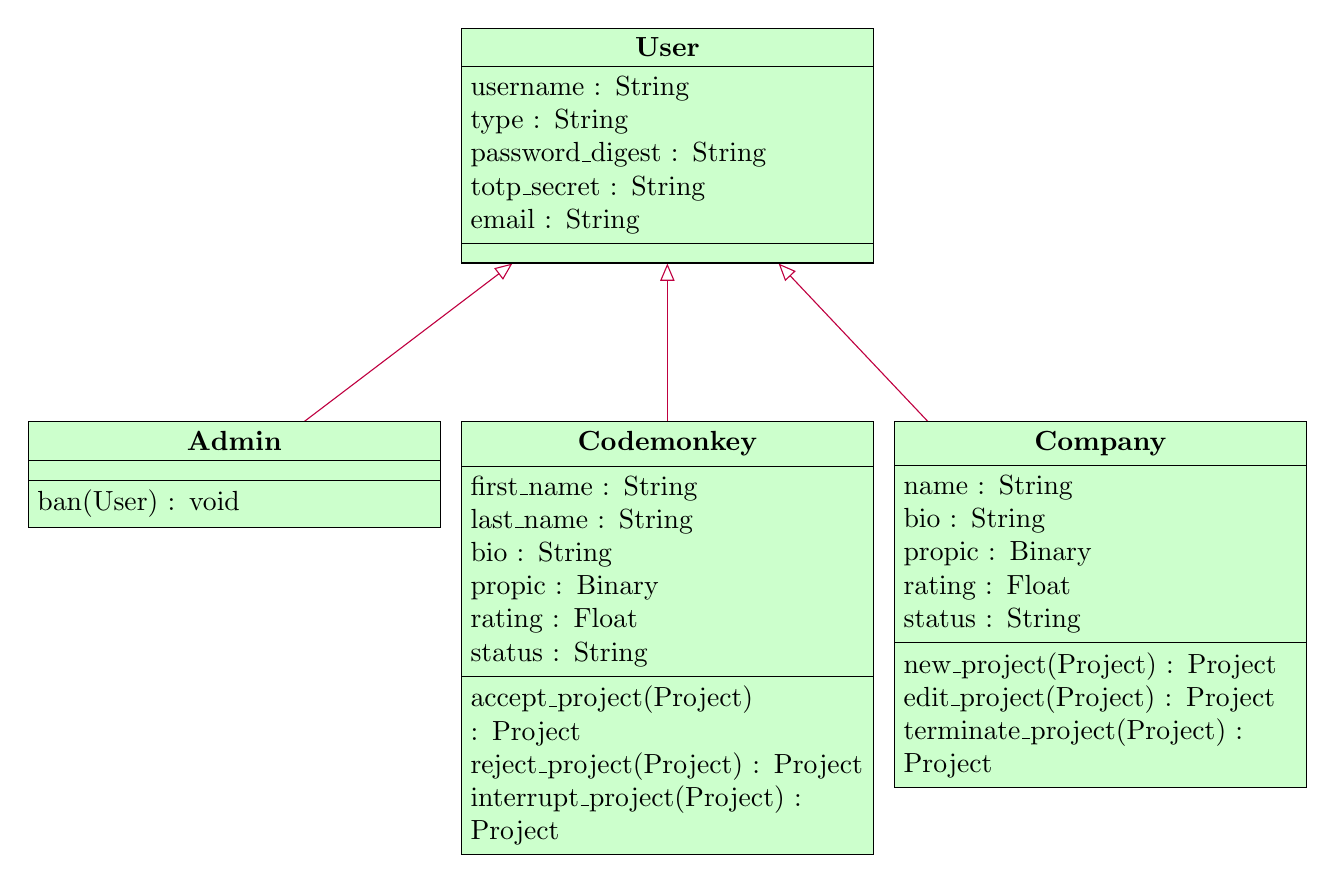
\begin{tikzpicture}

  \begin{class}[text width=5cm, fill=green!20, draw=black]{User}{0,0}
    \attribute{username : String}
    \attribute{type : String}
    \attribute{password\_digest : String}
    \attribute{totp\_secret : String}
    \attribute{email : String}
  \end{class}

  \begin{class}[text width=5cm, fill=green!20, draw=black]{Admin}{-5.5,-5}
    \inherit{User}
    \operation{ban(User) : void}
  \end{class}

  \begin{class}[text width=5cm, fill=green!20, draw=black]{Codemonkey}{0,-5}
    \inherit{User}
    \attribute{first\_name : String}
      \attribute{last\_name : String}
      \attribute{bio : String}
      \attribute{propic : Binary}
      \attribute{rating : Float}
      \attribute{status : String}
      \operation{accept\_project(Project) : Project}
      \operation{reject\_project(Project) : Project}
      \operation{interrupt\_project(Project) : Project}
  \end{class}

  \begin{class}[text width=5cm, fill=green!20, draw=black]{Company}{5.5,-5}
    \inherit{User}
      \attribute{name : String}
      \attribute{bio : String}
      \attribute{propic : Binary}
      \attribute{rating : Float}
      \attribute{status : String}
      \operation{new\_project(Project) : Project}
      \operation{edit\_project(Project) : Project}
      \operation{terminate\_project(Project) : Project}
  \end{class}

\end{tikzpicture}

\end{document}
